\chapter[Aufbau eines Computers]{Aufbau eines Computers}\label{ch:aufbau_computer}

\section{Überblick: Was ist ein Computer?}

Ein \tib{Computer}\index{Computer} (auch Rechner) ist eine Maschine, die nach einem gespeicherten Programm Daten verarbeitet. Er kann eingegebene Informationen in Ausgaben umwandeln -- sei es das Berechnen einer Summe, das Anzeigen eines Bildes oder das Abspielen von Musik. In \cref{ch:logische_gatter} haben wir gesehen, wie aus einzelnen Transistoren Gatter und aus Gattern einfache Rechenschaltungen wie der Halbaddierer entstehen. In diesem Kapitel setzen wir diese Bausteine zu einem vollständigen Computer zusammen. Grundlegend gilt dabei:

\begin{center}
    \begin{tikzpicture}[node distance=1.5cm]
    \node[draw, fill=RoyalBlue!15, minimum width=2.5cm, minimum height=1cm, rounded corners] (ein) {Eingabe};
    \node[draw, fill=Goldenrod!30, minimum width=2.5cm, minimum height=1cm, rounded corners, right=of ein] (ver) {Verarbeitung};
    \node[draw, fill=DarkSeaGreen!40, minimum width=2.5cm, minimum height=1cm, rounded corners, right=of ver] (aus) {Ausgabe};
    \draw[->, thick] (ein) -- (ver);
    \draw[->, thick] (ver) -- (aus);
\end{tikzpicture}

\end{center}

\section{Die Von-Neumann-Architektur}

Fast alle heute eingesetzten Rechner basieren auf dem Entwurf des Mathematikers John von Neumann aus dem Jahr 1945, der sogenannten \tib{Von-Neumann-Architektur}\index{Von-Neumann-Architektur}. Ihr entscheidendes Merkmal: \emph{Programm und Daten} werden im \emph{gleichen} Speicher abgelegt -- das Programm, das ein Computer ausführt, ist selbst ein Stück Daten (also eine Bitfolge, vgl. \cref{ch:kodierungen}), das jederzeit verändert oder ausgetauscht werden kann.

\begin{figure}[H]
    \centering
    \input{Grundlagen_Info/16_ComputerUndKodierungen/Figures/tikz_von_neumann.tex}
    \caption{Vereinfachtes Schaubild der Von-Neumann-Architektur.}
    \label{fig:von_neumann}
\end{figure}

Die Hauptkomponenten sind:

\begin{description}
    \item[\tib{\gls{CPU}}\index{CPU} (Central Processing Unit, Prozessor)] Führt die Anweisungen eines Programms aus. Enthält Steuerwerk, \gls{ALU} und Register.
    \item[\tib{Arbeitsspeicher (\gls{RAM})}\index{RAM}] Speichert aktuell laufende Programme und Daten. Der Inhalt geht beim Ausschalten verloren (\emph{flüchtig}).
    \item[\tib{Massenspeicher}\index{Massenspeicher}] Dauerhafte Ablage von Programmen und Dateien (\gls{HDD}, \gls{SSD}). Der Inhalt bleibt auch ohne Strom erhalten (\emph{nicht flüchtig}).
    \item[\tib{Ein-/Ausgabe}\index{Ein-/Ausgabe}] Verbindet den Computer mit der Aussenwelt: Tastatur, Maus, Bildschirm, Netzwerk, \gls{USB} usw.
    \item[\tib{Systembus}\index{Systembus}] Kommunikationskanal, über den alle Komponenten Daten und Steuersignale austauschen.
\end{description}

\subsection{Das mentale Modell: Die Büro-Analogie}

Um sich das Zusammenspiel und die spezifischen Rollen der Komponenten einzuprägen, hilft der Vergleich mit einem typischen Arbeitsplatz im Büro:

\begin{table}[H]
    \centering
    \resizebox{\textwidth}{!}{%
    \begin{tabular}{@{}lll@{}}
        \textbf{Komponente} & \textbf{Rolle im Büro / am Arbeitsplatz} & \textbf{Funktion im Computer} \\\midrule
        \textbf{\gls{CPU} (Prozessor)} & \textbf{Arbeitende Person} & Führt Programmbefehle schrittweise aus \\
        \quad $\hookrightarrow$ \textit{Steuerwerk} & Gehirn / Planer (liest Anleitung) & Decodiert Befehle, steuert Gesamtablauf und Takt \\
        \quad $\hookrightarrow$ \textit{\gls{ALU}} & Taschenrechner / Werkzeug in Händen & Führt Rechenoperationen und Vergleiche aus \\
        \quad $\hookrightarrow$ \textit{Register} & Notizblock / Hände unmittelbar vor sich & Schnellste, winzige Zwischenspeicher der \gls{CPU} \\
        \textbf{\gls{RAM} (Arbeitsspeicher)} & \textbf{Schreibtischplatte} & Schneller Zugriff; am Feierabend geleert (\emph{flüchtig}) \\
        \textbf{Massenspeicher (\gls{SSD}/\gls{HDD})} & \textbf{Aktenschrank / Archiv} & Grosse, dauerhafte Dateiablage (\emph{nicht flüchtig}) \\
        \textbf{Systembus} & \textbf{Laufwege / Förderband} & Verbindet alle Bereiche für schnellen Datentransfer \\
        \textbf{Ein-/Ausgabe (I/O)} & \textbf{Posteingang \& Fenster/Aushang} & Schnittstelle zur Aussenwelt (Tastatur, Monitor) \\
    \end{tabular}%
    }
    \caption{Die Büro-Analogie zur Veranschaulichung der Computerkomponenten.}
    \label{tab:computer_analogie}
\end{table}

\subsection{Vom Schema zur realen Hardware}

Auf der Hauptplatine (\tib{Mainboard}\index{Mainboard} bzw.\ \textit{Motherboard}) eines Computers sind diese theoretischen Komponenten als physische Bausteine angeordnet. Die Leiterbahnen auf der Platine bilden den Systembus, über den Daten zwischen Sockel, Speicherbänken und Anschlüssen fliessen (\cref{fig:mainboard_schema}).

\begin{figure}[H]
    \centering
    \providecommand{\mainboardHighlight}{all}

\tikzset{
    mbActive/.style={opacity=1.0, text opacity=1.0},
    mbDimmed/.style={opacity=0.18, text opacity=0.22}
}

\newcommand{\mbSetScope}[1]{%
    \tikzset{mbScope/.style={mbDimmed}}%
    \edef\mbCurVal{#1}%
    \edef\mbHLVal{\mainboardHighlight}%
    \ifx\mbHLVal\mbCurVal
        \tikzset{mbScope/.style={mbActive}}%
    \else
        \def\mbAllVal{all}%
        \ifx\mbHLVal\mbAllVal
            \tikzset{mbScope/.style={mbActive}}%
        \else
            \def\mbStorageVal{storage}\def\mbSSDVal{ssd}%
            \ifx\mbHLVal\mbStorageVal\ifx\mbCurVal\mbSSDVal\tikzset{mbScope/.style={mbActive}}\fi\fi
            \ifx\mbHLVal\mbSSDVal\ifx\mbCurVal\mbStorageVal\tikzset{mbScope/.style={mbActive}}\fi\fi
            \def\mbPCIeVal{pcie}\def\mbSlotsVal{slots}\def\mbBusVal{bus}%
            \ifx\mbHLVal\mbPCIeVal\ifx\mbCurVal\mbSlotsVal\tikzset{mbScope/.style={mbActive}}\fi\fi
            \ifx\mbHLVal\mbPCIeVal\ifx\mbCurVal\mbBusVal\tikzset{mbScope/.style={mbActive}}\fi\fi
            \ifx\mbHLVal\mbSlotsVal\ifx\mbCurVal\mbPCIeVal\tikzset{mbScope/.style={mbActive}}\fi\fi
            \ifx\mbHLVal\mbBusVal\ifx\mbCurVal\mbPCIeVal\tikzset{mbScope/.style={mbActive}}\fi\fi
            \ifx\mbHLVal\mbBusVal\ifx\mbCurVal\mbSlotsVal\tikzset{mbScope/.style={mbActive}}\fi\fi
        \fi
    \fi
}

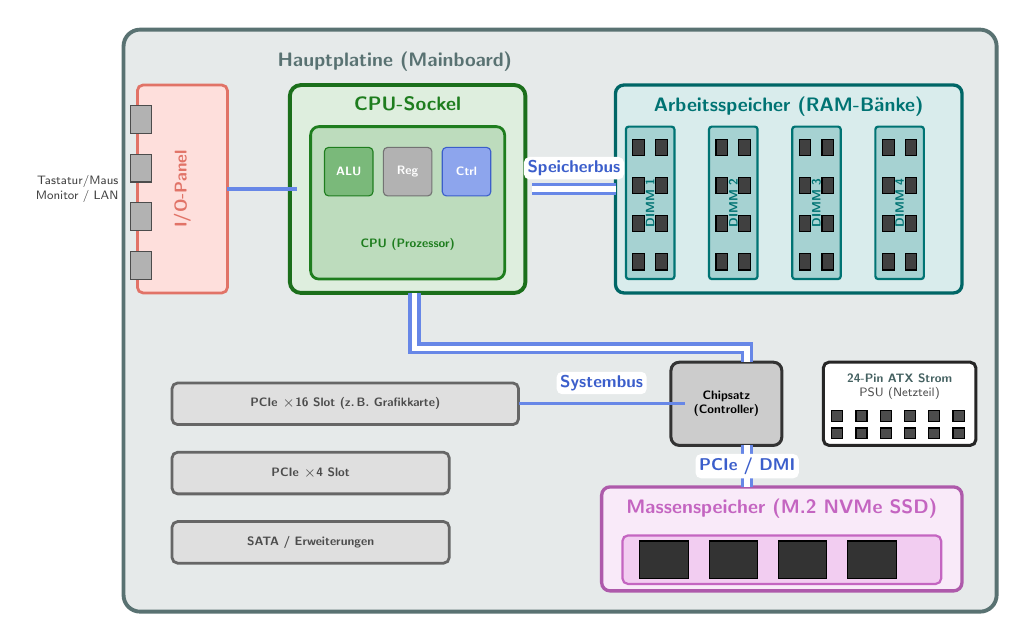
\begin{tikzpicture}[
    scale=0.88,
    every node/.style={transform shape},
    board/.style={fill=DarkSlateGray!12, draw=DarkSlateGray!80, line width=1.4pt, rounded corners=6pt},
    trace/.style={draw=RoyalBlue!80, line width=1.2pt},
    buslabel/.style={font=\scriptsize\bfseries\sffamily, text=RoyalBlue!90!black, fill=white, inner sep=1.5pt, rounded corners=2pt}
]
    % --- Mainboard Platine ---
    \def\mbAllVal{all}%
    \edef\mbHLVal{\mainboardHighlight}%
    \ifx\mbHLVal\mbAllVal
        \tikzset{mbBoardScope/.style={opacity=1.0, text opacity=1.0}}%
    \else
        \tikzset{mbBoardScope/.style={opacity=0.45, text opacity=0.55}}%
    \fi
    \begin{scope}[mbBoardScope]
        \draw[board] (-6.3, -4.2) rectangle (6.3, 4.2);
        \node[anchor=north west, font=\bfseries\sffamily\footnotesize, text=DarkSlateGray!80] at (-4.2, 4.0) {Hauptplatine (Mainboard)};
    \end{scope}

    % --- I/O Panel (links) ---
    \mbSetScope{io}
    \begin{scope}[mbScope]
        \draw[fill=Salmon!25, draw=Salmon!90!black, line width=1pt, rounded corners=2pt] (-6.1, 0.4) rectangle (-4.8, 3.4);
        \node[rotate=90, font=\bfseries\sffamily\scriptsize, text=Salmon!90!black] at (-5.45, 1.9) {I/O-Panel};
        \foreach \y in {0.8, 1.5, 2.2, 2.9} {
            \draw[fill=gray!60, draw=black!70] (-6.2, \y-0.2) rectangle (-5.9, \y+0.2);
        }
        \node[anchor=east, font=\tiny\sffamily, text=black!75, align=right] at (-6.25, 1.9) {Tastatur/Maus\\Monitor / LAN};
    \end{scope}

    % --- CPU Sockel & Prozessor (Mitte-Links) ---
    \mbSetScope{cpu}
    \begin{scope}[mbScope]
        \draw[fill=ForestGreen!15, draw=ForestGreen!80!black, line width=1.4pt, rounded corners=4pt] (-3.9, 0.4) rectangle (-0.5, 3.4);
        \node[anchor=north, font=\bfseries\sffamily\footnotesize, text=ForestGreen!90!black] at (-2.2, 3.35) {CPU-Sockel};

        % CPU Innenleben (ALU, Register, Steuerwerk)
        \draw[fill=ForestGreen!30, draw=ForestGreen!90!black, line width=1pt, rounded corners=3pt] (-3.6, 0.6) rectangle (-0.8, 2.8);
        
        % Sub-blocks
        \draw[fill=ForestGreen!60, draw=ForestGreen!90!black, rounded corners=1.5pt] (-3.4, 1.8) rectangle (-2.7, 2.5);
        \node[font=\tiny\bfseries\sffamily, text=white] at (-3.05, 2.15) {ALU};
        
        \draw[fill=Gray!60, draw=Gray!90!black, rounded corners=1.5pt] (-2.55, 1.8) rectangle (-1.85, 2.5);
        \node[font=\tiny\bfseries\sffamily, text=white] at (-2.2, 2.15) {Reg};
        
        \draw[fill=RoyalBlue!60, draw=RoyalBlue!90!black, rounded corners=1.5pt] (-1.7, 1.8) rectangle (-1.0, 2.5);
        \node[font=\tiny\bfseries\sffamily, text=white] at (-1.35, 2.15) {Ctrl};
        
        \node[font=\tiny\sffamily\bfseries, text=ForestGreen!90!black] at (-2.2, 1.1) {CPU (Prozessor)};
    \end{scope}

    % --- RAM Bänke (Rechts oben) ---
    \mbSetScope{ram}
    \begin{scope}[mbScope]
        \draw[fill=Teal!15, draw=Teal!80!black, line width=1.2pt, rounded corners=3pt] (0.8, 0.4) rectangle (5.8, 3.4);
        \node[anchor=north, font=\bfseries\sffamily\footnotesize, text=Teal!90!black] at (3.3, 3.35) {Arbeitsspeicher (RAM-Bänke)};

        % 4 RAM Riegel
        \foreach \x/\label in {1.3/DIMM 1, 2.5/DIMM 2, 3.7/DIMM 3, 4.9/DIMM 4} {
            \draw[fill=Teal!35, draw=Teal!90!black, line width=0.8pt, rounded corners=1pt] (\x-0.35, 0.6) rectangle (\x+0.35, 2.8);
            \node[rotate=90, font=\tiny\sffamily\bfseries, text=Teal!90!black] at (\x, 1.7) {\label};
            \foreach \y in {0.85, 1.4, 1.95, 2.5} {
                \draw[fill=black!75] (\x-0.25, \y-0.12) rectangle (\x-0.08, \y+0.12);
                \draw[fill=black!75] (\x+0.08, \y-0.12) rectangle (\x+0.25, \y+0.12);
            }
        }
    \end{scope}

    % --- Chipsatz (Mitte) ---
    \mbSetScope{chipset}
    \begin{scope}[mbScope]
        \draw[fill=gray!40, draw=black!80, line width=1.1pt, rounded corners=3pt] (1.6, -1.8) rectangle (3.2, -0.6);
        \node[font=\tiny\sffamily\bfseries, text=black, align=center] at (2.4, -1.2) {Chipsatz\\(Controller)};
    \end{scope}

    % --- 24-Pin ATX Stromanschluss (Netzteil / PSU) (Mitte-Rechts) ---
    \mbSetScope{psu}
    \begin{scope}[mbScope]
        \draw[fill=white, draw=black!85, line width=1.1pt, rounded corners=2pt] (3.8, -1.8) rectangle (6.0, -0.6);
        \node[anchor=north, font=\tiny\bfseries\sffamily, text=DarkSlateGray!90] at (4.9, -0.65) {24-Pin ATX Strom};
        \foreach \px in {4.0, 4.35, 4.7, 5.05, 5.4, 5.75} {
            \draw[fill=black!70] (\px-0.08, -1.45) rectangle (\px+0.08, -1.3);
            \draw[fill=black!70] (\px-0.08, -1.7) rectangle (\px+0.08, -1.55);
        }
        \node[font=\tiny\sffamily, text=black!70] at (4.9, -1.05) {\glsentryshort{PSU} (Netzteil)};
    \end{scope}

    % --- Massenspeicher (M.2 NVMe SSD) (Rechts unten) ---
    \mbSetScope{storage}
    \begin{scope}[mbScope]
        \draw[fill=Orchid!15, draw=Orchid!80!black, line width=1.2pt, rounded corners=3pt] (0.6, -3.9) rectangle (5.8, -2.4);
        \node[anchor=north, font=\bfseries\sffamily\footnotesize, text=Orchid!90!black] at (3.2, -2.45) {Massenspeicher (M.2 NVMe SSD)};
        \draw[fill=Orchid!35, draw=Orchid!90!black, line width=0.8pt, rounded corners=2pt] (0.9, -3.8) rectangle (5.5, -3.1);
        \foreach \cx in {1.5, 2.5, 3.5, 4.5} {
            \draw[fill=black!80] (\cx-0.35, -3.72) rectangle (\cx+0.35, -3.18);
        }
    \end{scope}

    % --- PCIe Steckplätze (Links unten) ---
    \mbSetScope{pcie}
    \begin{scope}[mbScope]
        \draw[fill=gray!25, draw=black!60, line width=1pt, rounded corners=2pt] (-5.6, -1.5) rectangle (-0.6, -0.9);
        \node[font=\tiny\bfseries\sffamily, text=black!70] at (-3.1, -1.2) {PCIe $\times$16 Slot (z.\,B. Grafikkarte)};
        \draw[fill=gray!25, draw=black!60, line width=1pt, rounded corners=2pt] (-5.6, -2.5) rectangle (-1.6, -1.9);
        \node[font=\tiny\bfseries\sffamily, text=black!70] at (-3.6, -2.2) {PCIe $\times$4 Slot};
        \draw[fill=gray!25, draw=black!60, line width=1pt, rounded corners=2pt] (-5.6, -3.5) rectangle (-1.6, -2.9);
        \node[font=\tiny\bfseries\sffamily, text=black!70] at (-3.6, -3.2) {SATA / Erweiterungen};
    \end{scope}

    % --- Systembus (Leiterbahnen) ---
    \mbSetScope{bus}
    \begin{scope}[mbScope]
        % CPU <-> RAM (Speicherbus)
        \draw[trace, double distance=2pt] (-0.4, 1.9) -- (0.8, 1.9);
        \node[buslabel] at (0.2, 2.2) {Speicherbus};

        % CPU <-> I/O Panel
        \draw[trace] (-3.8, 1.9) -- (-4.8, 1.9);

        % CPU <-> Chipsatz
        \draw[trace, double distance=2pt] (-2.1, 0.4) -- (-2.1, -0.4) -- (2.7, -0.4) -- (2.7, -0.6);
        
        % Chipsatz <-> M.2 SSD
        \draw[trace, double distance=2pt] (2.7, -1.8) -- (2.7, -2.4);
        \node[buslabel] at (2.7, -2.1) {PCIe / DMI};

        % Chipsatz <-> PCIe Slots
        \draw[trace] (1.8, -1.2) -- (-0.6, -1.2);
        \node[buslabel] at (0.6, -0.9) {Systembus};
    \end{scope}
\end{tikzpicture}

    \caption{Stilisierter Aufbau eines Mainboards mit den Hauptkomponenten.}
    \label{fig:mainboard_schema}
\end{figure}

\begin{figure}[H]
    \centering
    \begin{subfigure}{0.48\textwidth}
        \centering
        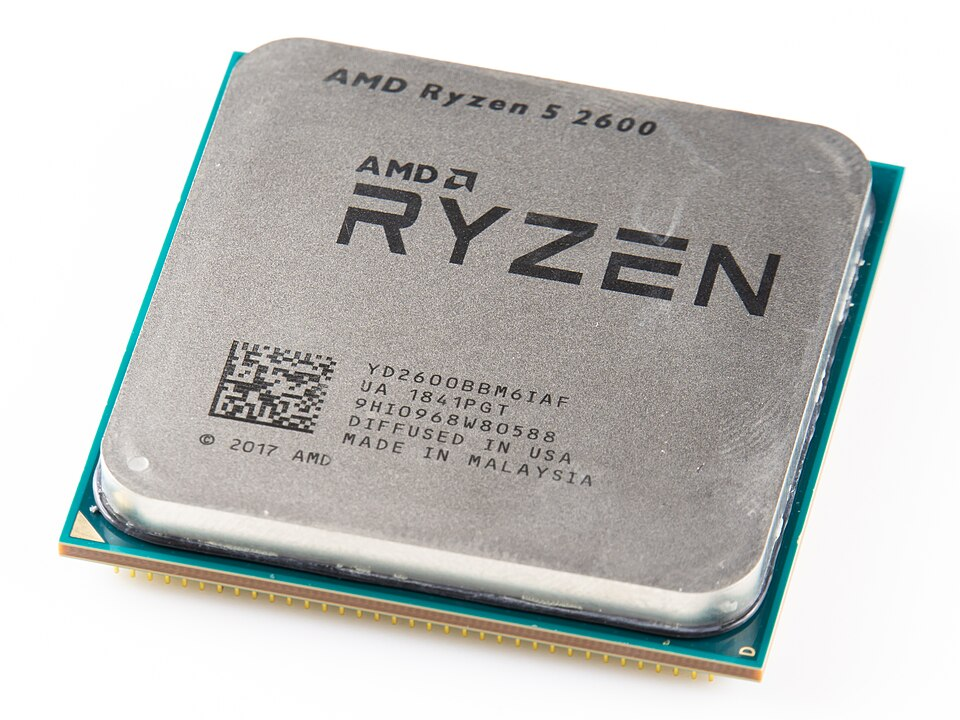
\includegraphics[width=0.88\linewidth,height=3.8cm,keepaspectratio]{Grundlagen_Info/16_ComputerUndKodierungen/Figures/cpu.jpg}
        \caption{\gls{CPU} (AMD Ryzen Prozessor mit Heatspreader). \href{https://commons.wikimedia.org/wiki/File:AMD_Ryzen_5_2600_(39851733273).jpg}{\color{RoyalBlue}\scriptsize[Quelle: Fritzchens Fritz, CC0]}}
        \label{fig:foto_cpu}
    \end{subfigure}\hfill
    \begin{subfigure}{0.48\textwidth}
        \centering
        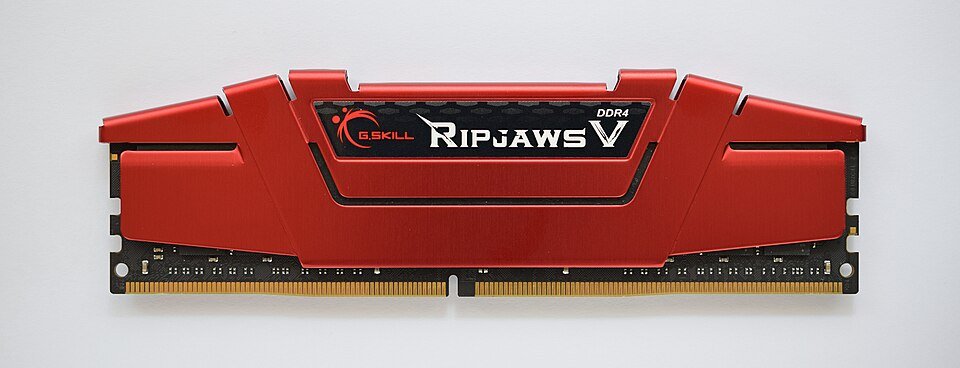
\includegraphics[width=0.88\linewidth,height=3.8cm,keepaspectratio]{Grundlagen_Info/16_ComputerUndKodierungen/Figures/ram.jpg}
        \caption{\gls{RAM} (DDR4-Arbeitsspeicher-Riegel). \href{https://commons.wikimedia.org/wiki/File:RAM_Module_(SDRAM-DDR4).jpg}{\color{RoyalBlue}\scriptsize[Quelle: ElooKoN, CC BY-SA 4.0]}}
        \label{fig:foto_ram}
    \end{subfigure}
    
    \vspace{0.8em}
    
    \begin{subfigure}{0.48\textwidth}
        \centering
        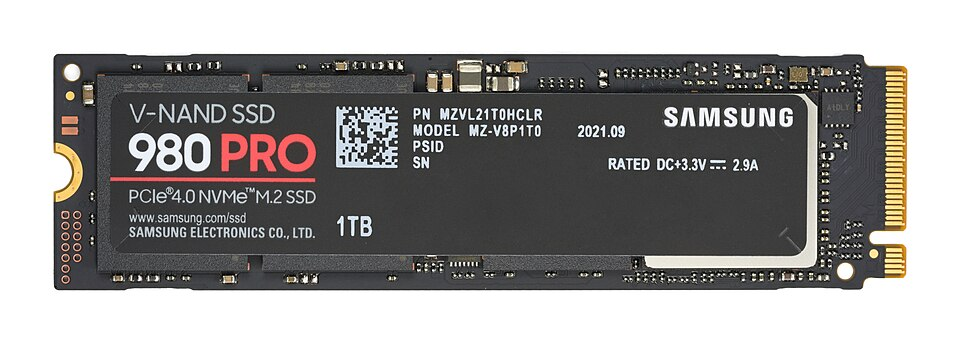
\includegraphics[width=0.88\linewidth,height=3.8cm,keepaspectratio]{Grundlagen_Info/16_ComputerUndKodierungen/Figures/ssd.jpg}
        \caption{Massenspeicher (M.2 \gls{NVMe} \gls{SSD}). \href{https://commons.wikimedia.org/wiki/File:Samsung_980_PRO_PCIe_4.0_NVMe_SSD_1TB-top_PNr\%C2\%B00915.jpg}{\color{RoyalBlue}\scriptsize[Quelle: D-Kuru, CC BY-SA 4.0]}}
        \label{fig:foto_ssd}
    \end{subfigure}\hfill
    \begin{subfigure}{0.48\textwidth}
        \centering
        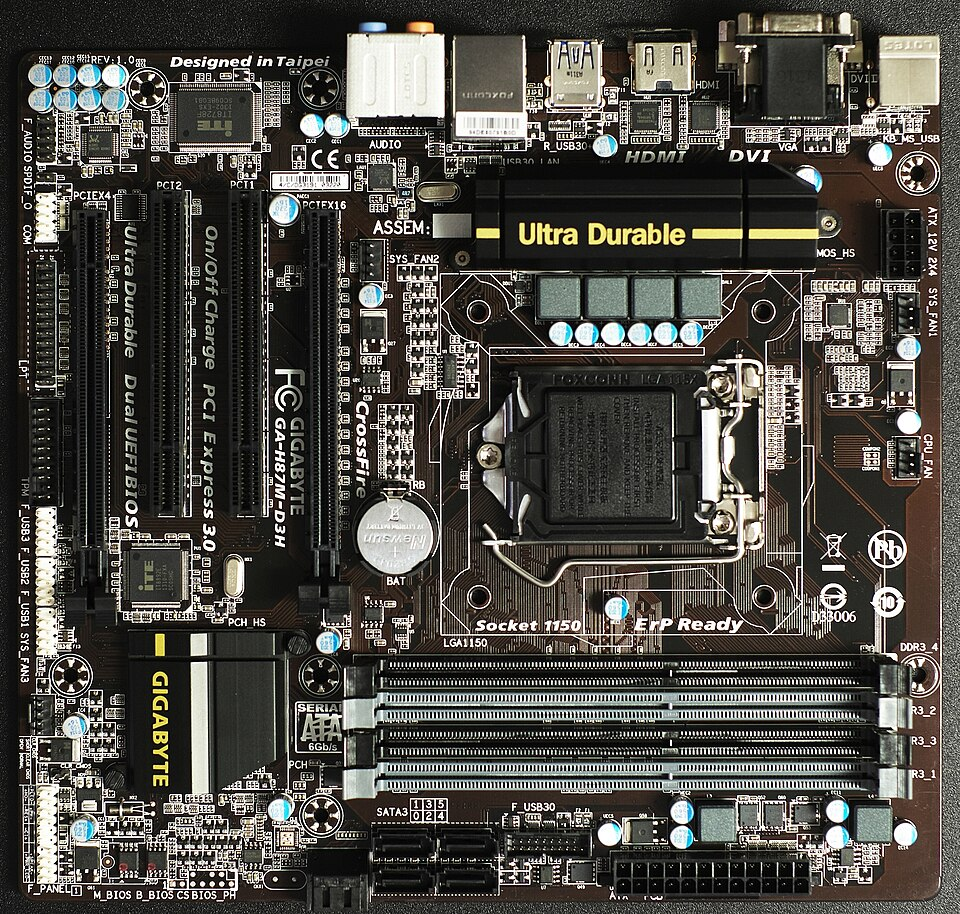
\includegraphics[width=0.88\linewidth,height=3.8cm,keepaspectratio]{Grundlagen_Info/16_ComputerUndKodierungen/Figures/mainboard.jpg}
        \caption{Mainboard (ATX-Hauptplatine). \href{https://commons.wikimedia.org/wiki/File:Gigabyte_GA-H87M-D3H_motherboard_\%C2\%B5ATX_with_Intel_Socket_1150.jpg}{\color{RoyalBlue}\scriptsize[Quelle: Gigabyte, FAL/CC BY-SA]}}
        \label{fig:foto_mainboard}
    \end{subfigure}
    \caption{Reale Hardware-Komponenten eines modernen Computers.}
    \label{fig:echte_hardware}
\end{figure}

\begin{myexercise}
    Ordnen Sie jeder Computerkomponente die passende Aufgabe zu. Verbinden Sie dazu die Begriffe (1--5) mit den Beschreibungen (A--E).
    \begin{center}
        \begin{tabular}{ll}
            \textbf{Komponente} & \textbf{Beschreibung} \\\midrule
            1. \gls{CPU} & A. Verbindet den Computer mit Tastatur, Bildschirm und Netzwerk \\
            2. Arbeitsspeicher (\gls{RAM}) & B. Führt die Anweisungen eines Programms aus \\
            3. Massenspeicher & C. Speichert aktuell benötigte Programme und Daten vorübergehend \\
            4. Ein-/Ausgabe & D. Überträgt Daten und Steuersignale zwischen den Komponenten \\
            5. Systembus & E. Speichert Programme und Dateien dauerhaft \\
        \end{tabular}
    \end{center}
    \begin{myanswer}
        1--B, 2--C, 3--E, 4--A, 5--D.
    \end{myanswer}
\end{myexercise}

\begin{myremark}[Von Neumann vs.\ heute]
    Heutige Prozessoren weichen in Details von Neumann ab (z.\,B. mehrere Kerne, Caches, getrennte Busse für Daten und Instruktionen), folgen aber dem grundlegenden Prinzip des gespeicherten Programms.
\end{myremark}




\begin{myexercise}
    Warum ist es problematisch, wenn Programm und Daten im \emph{gleichen} Speicher liegen? Überlegen Sie, was passieren könnte, wenn ein fehlerhaftes Programm versehentlich in den Speicherbereich schreibt, in dem sein eigener Programmcode liegt.
    \begin{myanswer}
        Ein Programm könnte theoretisch seinen eigenen (oder einen fremden) Programmcode überschreiben, was zu unvorhersehbarem Verhalten oder einem Absturz führt. Aus diesem Grund übernimmt das Betriebssystem (siehe \cref{ch:betriebssystem}) die Aufgabe, den Speicherbereich verschiedener Programme voneinander zu isolieren (\tib{Speicherschutz}).
    \end{myanswer}
\end{myexercise}

\section{Die \gls{CPU} im Detail}

\subsection{\gls{ALU} -- Arithmetisch-logische Einheit}

Die \tib{\gls{ALU}}\index{ALU} (englisch: \emph{Arithmetic Logic Unit}) ist das \enquote{Rechenzentrum} der \gls{CPU}. Sie führt arithmetische Operationen (Addition, Subtraktion, \ldots) und logische Operationen (AND, OR, Vergleiche, \ldots) auf Binärzahlen aus. Intern besteht sie -- wie in \cref{ch:logische_gatter} gesehen -- aus einer grossen Anzahl kombinierter Logikgatter, zum Beispiel Volladdierern (vgl. \cref{sec:halbaddierer}).

\subsection{Steuerwerk}

Das \tib{Steuerwerk}\index{Steuerwerk} (englisch: \emph{control unit}) steuert den Ablauf aller Operationen. Es liest Befehle aus dem Speicher, interpretiert sie und gibt der \gls{ALU} und den übrigen Komponenten die entsprechenden Steuersignale.

\subsection{Register}

\tib{Register}\index{Register} sind sehr schnelle, aber winzige Zwischenspeicher direkt in der \gls{CPU}. Sie halten die Werte, mit denen die \gls{ALU} gerade rechnet (z.\,B. die zwei Summanden und das Resultat einer Addition). Typische Grösse: 64~Bit pro Register -- also 8 Byte (vgl. \cref{mydefinition:bit-byte}).

\section{Arbeitsspeicher (\gls{RAM})}

Der \tib{\gls{RAM}}\index{RAM} (englisch: \emph{Random Access Memory}) speichert alle Programme und Daten, die der Computer im Moment benötigt. Man kann sich den \gls{RAM} als eine lange Tabelle vorstellen, in der jede Zeile einer \tib{Speicherzelle}\index{Speicherzelle} entspricht und eine eindeutige \tib{Adresse}\index{Adresse} hat:

\begin{table}[H]
    \centering
    \begin{tabular}{cc}
        \textbf{Adresse} & \textbf{Inhalt (1 Byte)} \\\midrule\midrule
        \texttt{0x00} & \texttt{10110100} \\\midrule
        \texttt{0x01} & \texttt{00001111} \\\midrule
        \texttt{0x02} & \texttt{11001010} \\\midrule
        $\vdots$ & $\vdots$ \\
    \end{tabular}
    \caption{Schematische Darstellung des \gls{RAM}: jede Adresse zeigt auf eine Speicherzelle von einem Byte. Die Notation \texttt{0x} kennzeichnet hexadezimale Adressen.}
    \label{tab:ram}
\end{table}

\begin{myattention}
    Die Adressen in \cref{tab:ram} sind in \tib{hexadezimaler Schreibweise}\index{Hexadezimalsystem} angegeben (vgl. \cref{section:stellenwertdarst}) -- daher das Präfix \texttt{0x}. Hexadezimalzahlen eignen sich hier besonders gut, da zwei Hex-Ziffern genau einem Byte entsprechen (vgl. \cref{ex:byte-max}).
\end{myattention}

Typische Grössen heutiger Rechner: 8--64~GB \gls{RAM} (vgl. \cref{table:daten-groessenordnungen}). Der \tib{Cache}\index{Cache} ist ein noch schnellerer, aber viel kleinerer Pufferspeicher in der \gls{CPU}, der häufig benötigte Daten zwischenspeichert, um den langsameren \gls{RAM} zu entlasten.

\subsection{Exkurs: \glsentryshort{SI}-Präfixe und Grössenordnungen in der Informatik}

Das \tib{\gls{SI}}\index{Internationales Einheitensystem (SI)} (\emph{Système international d'unités}, französisch für internationales Einheitensystem) ist das weltweit am weitesten verbreitete und standardisierte Einheitensystem für physikalische Grössen (wie die Sekunde für Zeitdauern oder das Hertz für Schwingungsfrequenzen). Um sehr grosse oder extrem kleine Zahlenwerte kompakt und lesbar darzustellen, definiert das \gls{SI} genormte Vorsätze (Präfixe) auf Basis von Zehnerpotenzen.

In der Informatik begegnen uns sowohl extrem kleine Einheiten (z.\,B.\ Nanosekunden bei \gls{CPU}-Takten und \gls{RAM}-Latenzen) als auch gewaltige Datenmengen (Gigabytes und Terabytes). Zur Orientierung und Umrechnung fasst \cref{table:daten-groessenordnungen} die standardisierten \gls{SI}-Vorsätze zusammen:

\begin{table}[H]
    \centering
    \resizebox{\textwidth}{!}{%
    \begin{tabular}{@{}lllll@{}}
        \textbf{Präfix} & \textbf{Symbol} & \textbf{Faktor (Zehnerpotenz)} & \textbf{Bedeutung} & \textbf{Typisches Beispiel in der Informatik} \\\midrule
        \multicolumn{5}{@{}l}{\textit{\textbf{Kleine Einheiten (Zeit, Latenz, Taktzyklen)}}} \\\midrule
        Nano & $\mathrm{n}$ & $10^{-9} = 0{,}000\,000\,001$ & Milliardstel & \gls{CPU}-Taktzyklus ($1\,\mathrm{GHz} \leftrightarrow 1\,\mathrm{ns}$), \gls{RAM}-Zugriff ($10\text{--}50\,\mathrm{ns}$) \\
        Mikro & $\mu$ & $10^{-6} = 0{,}000\,001$ & Millionstel & \gls{SSD}-Latenz ($20\text{--}100\,\mu\mathrm{s}$), Interrupt-Reaktionszeit \\
        Milli & $\mathrm{m}$ & $10^{-3} = 0{,}001$ & Tausendstel & \gls{HDD}-Latenz ($5\text{--}15\,\mathrm{ms}$), Netzwerk-Ping ($10\text{--}50\,\mathrm{ms}$) \\\midrule
        \multicolumn{5}{@{}l}{\textit{\textbf{Grosse Einheiten (Speicherkapazitäten, Übertragungsraten, Taktfrequenzen)}}} \\\midrule
        Kilo & $\mathrm{k}$ & $10^3 = 1\,000$ & Tausend & Textdatei / Icon ($50\,\mathrm{kB}$), $1\,\mathrm{kHz}$ Frequenz \\
        Mega & $\mathrm{M}$ & $10^6 = 1\,000\,000$ & Million & Foto / MP3-Song ($5\text{--}25\,\mathrm{MB}$), \gls{HDD}-Rate ($150\,\mathrm{MB/s}$) \\
        Giga & $\mathrm{G}$ & $10^9 = 1\,000\,000\,000$ & Milliarde & \gls{RAM} ($16\,\mathrm{GB}$), \gls{CPU}-Takt ($3{,}6\,\mathrm{GHz}$), \gls{SSD}-Rate ($7\,\mathrm{GB/s}$) \\
        Tera & $\mathrm{T}$ & $10^{12} = 1\,000\,000\,000\,000$ & Billion & \gls{SSD}-/\gls{HDD}-Massenspeicher ($1\text{--}4\,\mathrm{TB}$) \\
        Peta & $\mathrm{P}$ & $10^{15} = 1\,000\,000\,000\,000\,000$ & Billiarde & Grosse Rechenzentren, Cloud-Datenspeicher \\
    \end{tabular}%
    }
    \caption{Übersicht der gebräuchlichen \gls{SI}-Präfixe für Zeiten, Frequenzen und Datenmengen.}
    \label{table:daten-groessenordnungen}
\end{table}

\begin{myremark}[Dezimal- vs.\ Binärpräfixe bei Datenmengen]
    Im \gls{SI}-System steht $\mathrm{k}$ exakt für $10^3 = 1\,000$ und $\mathrm{M}$ für $10^6 = 1\,000\,000$. Historisch wurde in der Informatik wegen der Zweierpotenzen oft mit $2^{10} = 1024$ gerechnet. Zur eindeutigen Unterscheidung wurden die \tib{Binärpräfixe}\index{Binärpräfixe} Kibi- ($\mathrm{KiB} = 1024\,\mathrm{B}$), Mebi- ($\mathrm{MiB} = 1024^2\,\mathrm{B}$) und Gibibyte ($\mathrm{GiB} = 1024^3\,\mathrm{B}$) genormt (IEC 60027-2). Bei Speicherherstellern und im Schulunterricht wird üblicherweise die dezimale \gls{SI}-Norm ($1\,\mathrm{GB} = 1000\,\mathrm{MB} = 10^9\,\mathrm{B}$) verwendet.
\end{myremark}

\begin{myexercise}\label{myexercise:si-praefixe-umwandlung}
    \textbf{Mini-Übung: Unhandliche Zahlen mit \glsentryshort{SI}-Präfixen lesbar machen.}
    In technischen Datenblättern und Programmen stösst man oft auf unübersichtliche Zahlen ohne Einheitsvorsätze. Wandeln Sie folgende Angaben in eine lesbare Form mit dem jeweils passendsten \gls{SI}-Präfix um:
    \begin{enumerate}[(a)]\setlength\itemsep{2pt}
        \item \textbf{\gls{RAM}-Lesezugriff:} $0{,}000\,000\,015\,\mathrm{s}$
        \item \textbf{\gls{NVMe}-\gls{SSD}-Latenz:} $0{,}000\,04\,\mathrm{s}$
        \item \textbf{\gls{CPU}-Taktfrequenz:} $3\,600\,000\,000\,\mathrm{Hz}$
        \item \textbf{System-Update (Dateigrösse):} $4\,800\,000\,000\,\mathrm{Byte}$
        \item \textbf{Backup-Server (Kapazität):} $12\,000\,000\,000\,000\,\mathrm{Byte}$
    \end{enumerate}

    \begin{myanswer}
        \begin{enumerate}[(a)]\setlength\itemsep{2pt}
            \item $0{,}000\,000\,015\,\mathrm{s} = 15 \times 10^{-9}\,\mathrm{s} = \mathbf{15\,\mathrm{ns}}$ (Nanosekunden).
            \item $0{,}000\,04\,\mathrm{s} = 40 \times 10^{-6}\,\mathrm{s} = \mathbf{40\,\mu\mathrm{s}}$ (Mikrosekunden).
            \item $3\,600\,000\,000\,\mathrm{Hz} = 3{,}6 \times 10^9\,\mathrm{Hz} = \mathbf{3{,}6\,\mathrm{GHz}}$ (Gigahertz).
            \item $4\,800\,000\,000\,\mathrm{Byte} = 4{,}8 \times 10^9\,\mathrm{Byte} = \mathbf{4{,}8\,\mathrm{GB}}$ (Gigabyte).
            \item $12\,000\,000\,000\,000\,\mathrm{Byte} = 12 \times 10^{12}\,\mathrm{Byte} = \mathbf{12\,\mathrm{TB}}$ (Terabyte).
        \end{enumerate}
    \end{myanswer}
\end{myexercise}

\section{Massenspeicher}

Während der Arbeitsspeicher (\gls{RAM}) Daten nur flüchtig speichert, dient der \tib{Massenspeicher} zur dauerhaften Sicherung von Betriebssystem, Programmen und Dateien. In modernen Computern kommen heute vor allem zwei Technologien zum Einsatz:

\begin{description}
    \item[\tib{\gls{HDD}}\index{HDD} (Hard Disk Drive)] Magnetische Metallscheiben (\textit{Platter}) rotieren mit mehreren tausend Umdrehungen pro Minute. Ein beweglicher Lese-/Schreibarm schwebt auf einem winzigen Luftpolster über den Scheiben und liest oder magnetisiert Bereiche auf der Oberfläche.
    \item[\tib{\gls{SSD}}\index{SSD} (Solid State Drive)] Reine Halbleitertechnik ohne bewegliche mechanische Bauteile. Die Daten werden in Form elektrischer Ladung in nicht-flüchtigen Flash-Speicherzellen (NAND-Flash) abgelegt und von einem integrierten Speichercontroller gesteuert.
\end{description}

\begin{figure}[H]
    \centering
    \begin{subfigure}{0.48\textwidth}
        \centering
        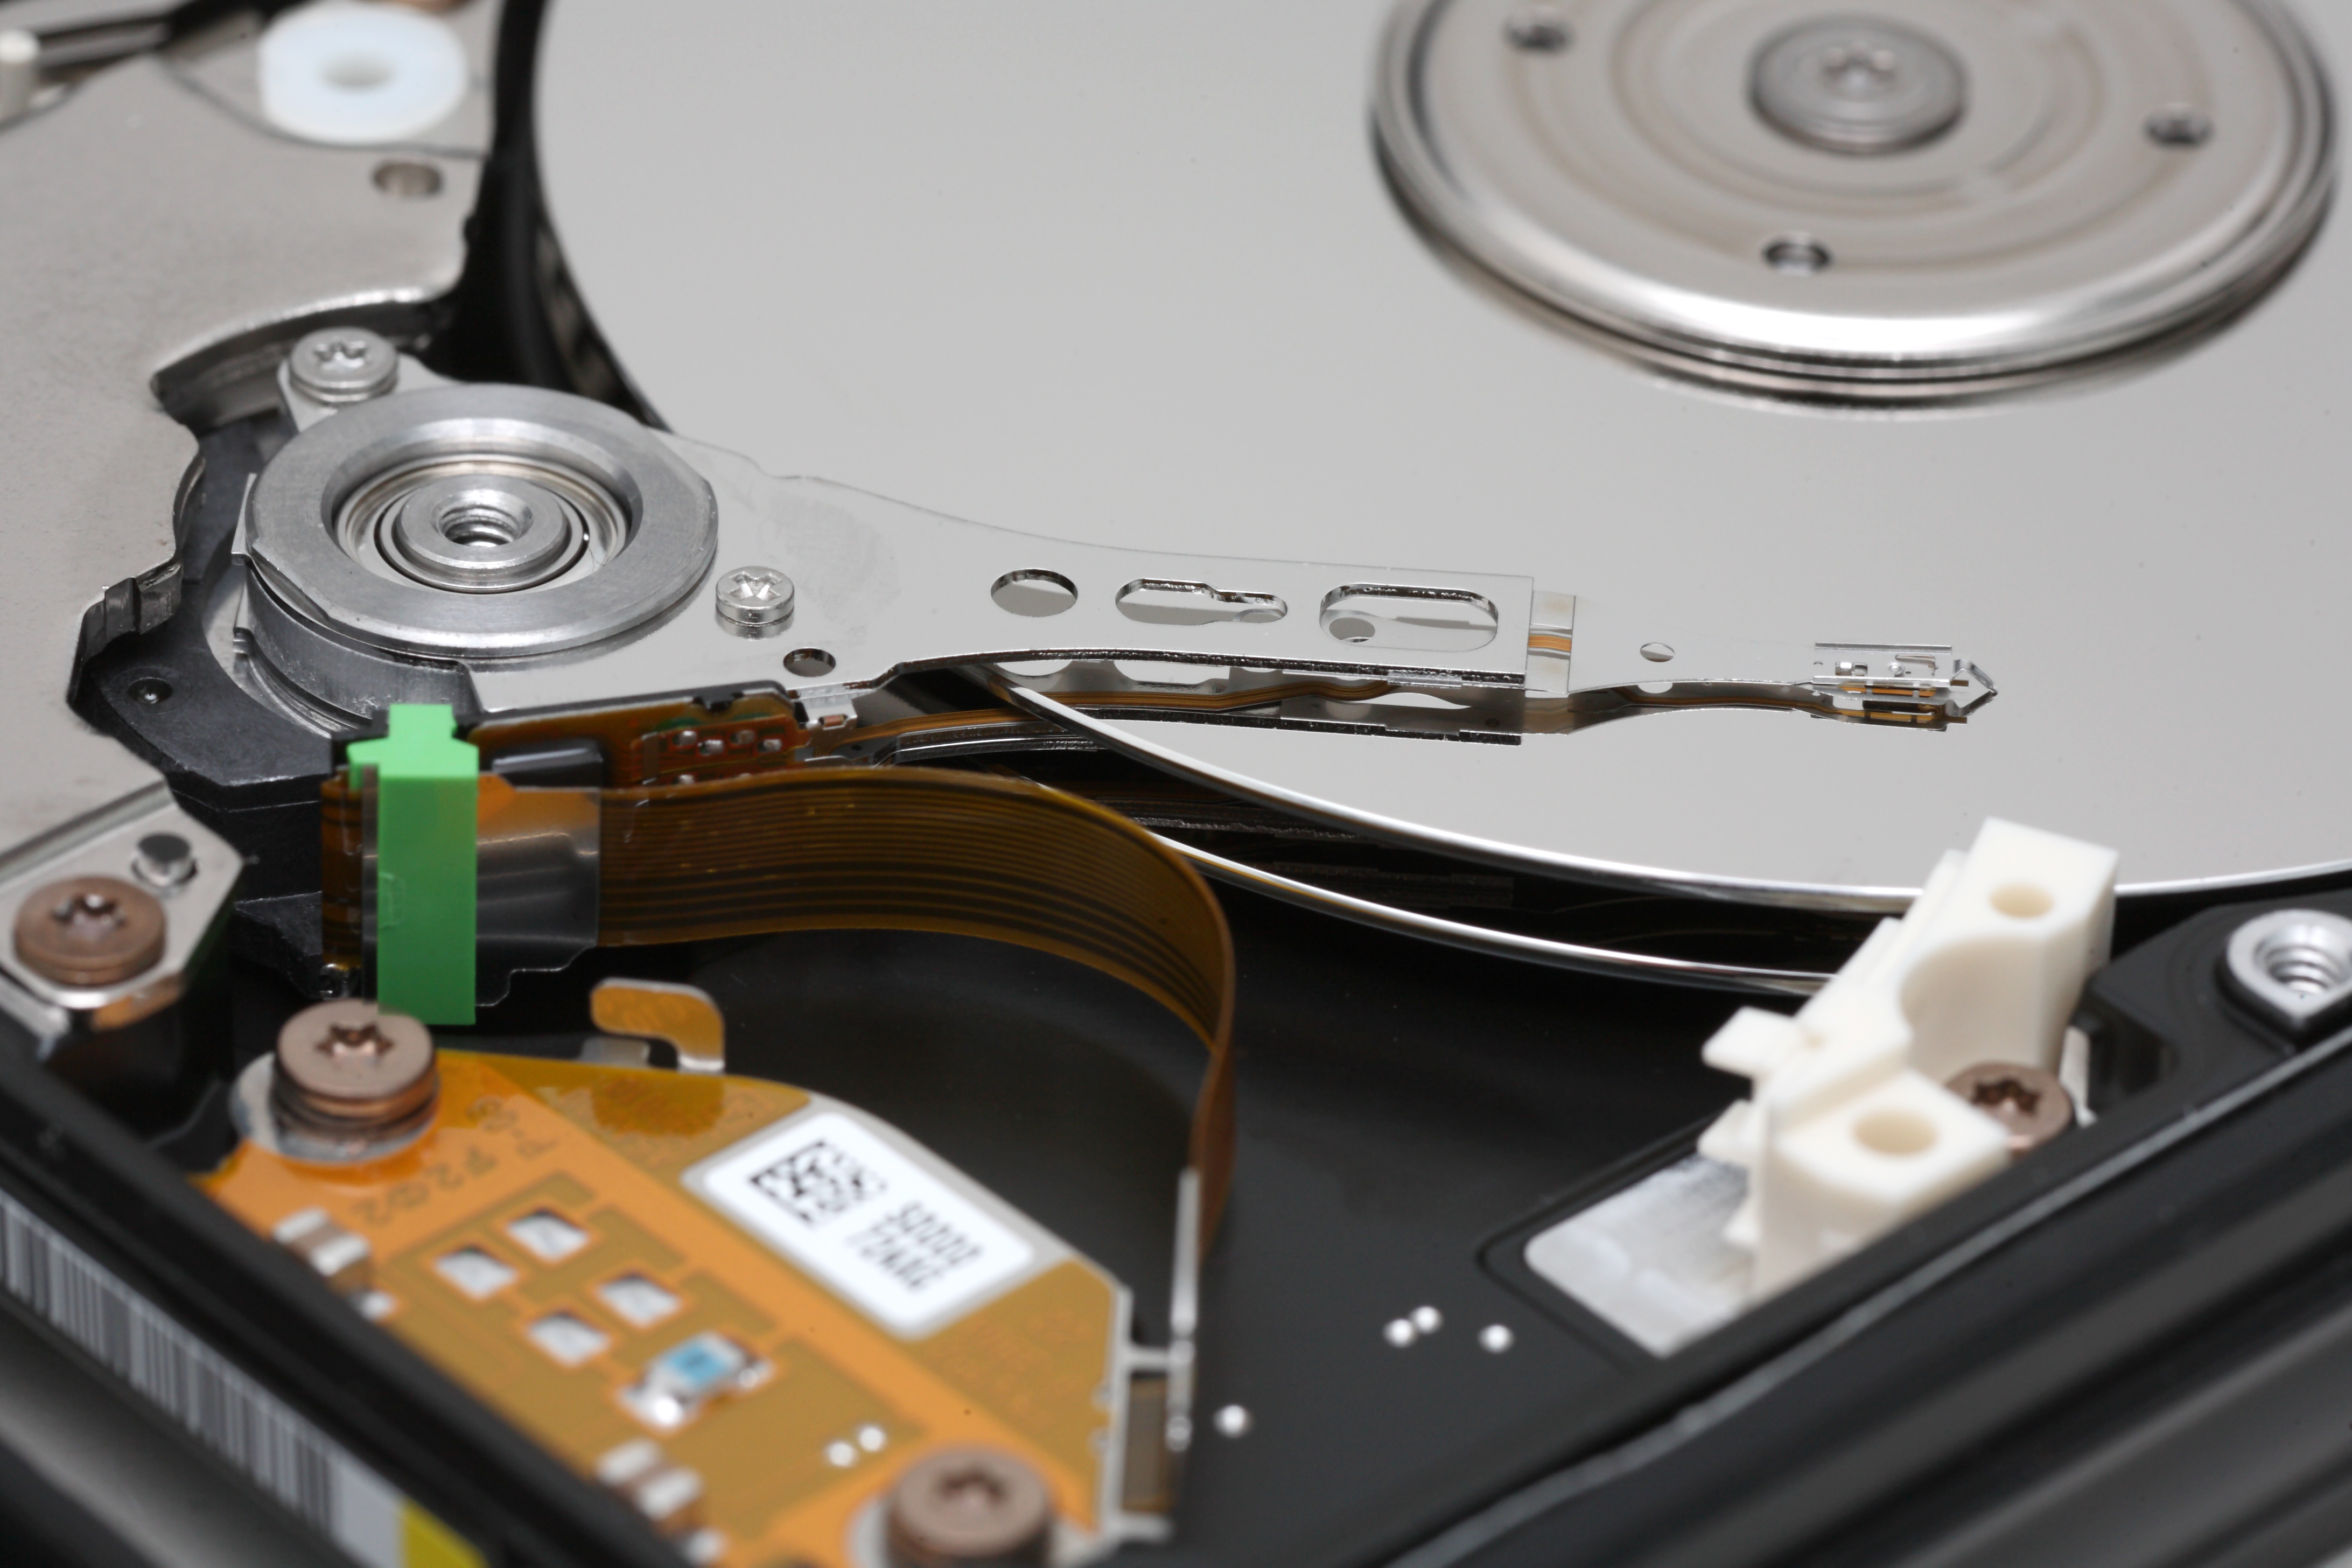
\includegraphics[width=0.88\linewidth,height=3.8cm,keepaspectratio]{Grundlagen_Info/16_ComputerUndKodierungen/Figures/hdd_inside.jpg}
        \caption{Geöffnete \gls{HDD}: rotierende Magnetscheiben und mechanischer Lese-/Schreibarm. \href{https://commons.wikimedia.org/wiki/File:Hard_disk_platters_and_head.jpg}{\color{RoyalBlue}\scriptsize[Quelle: M.\ Field, CC BY-SA 3.0]}}
        \label{fig:foto_hdd_inside}
    \end{subfigure}\hfill
    \begin{subfigure}{0.48\textwidth}
        \centering
        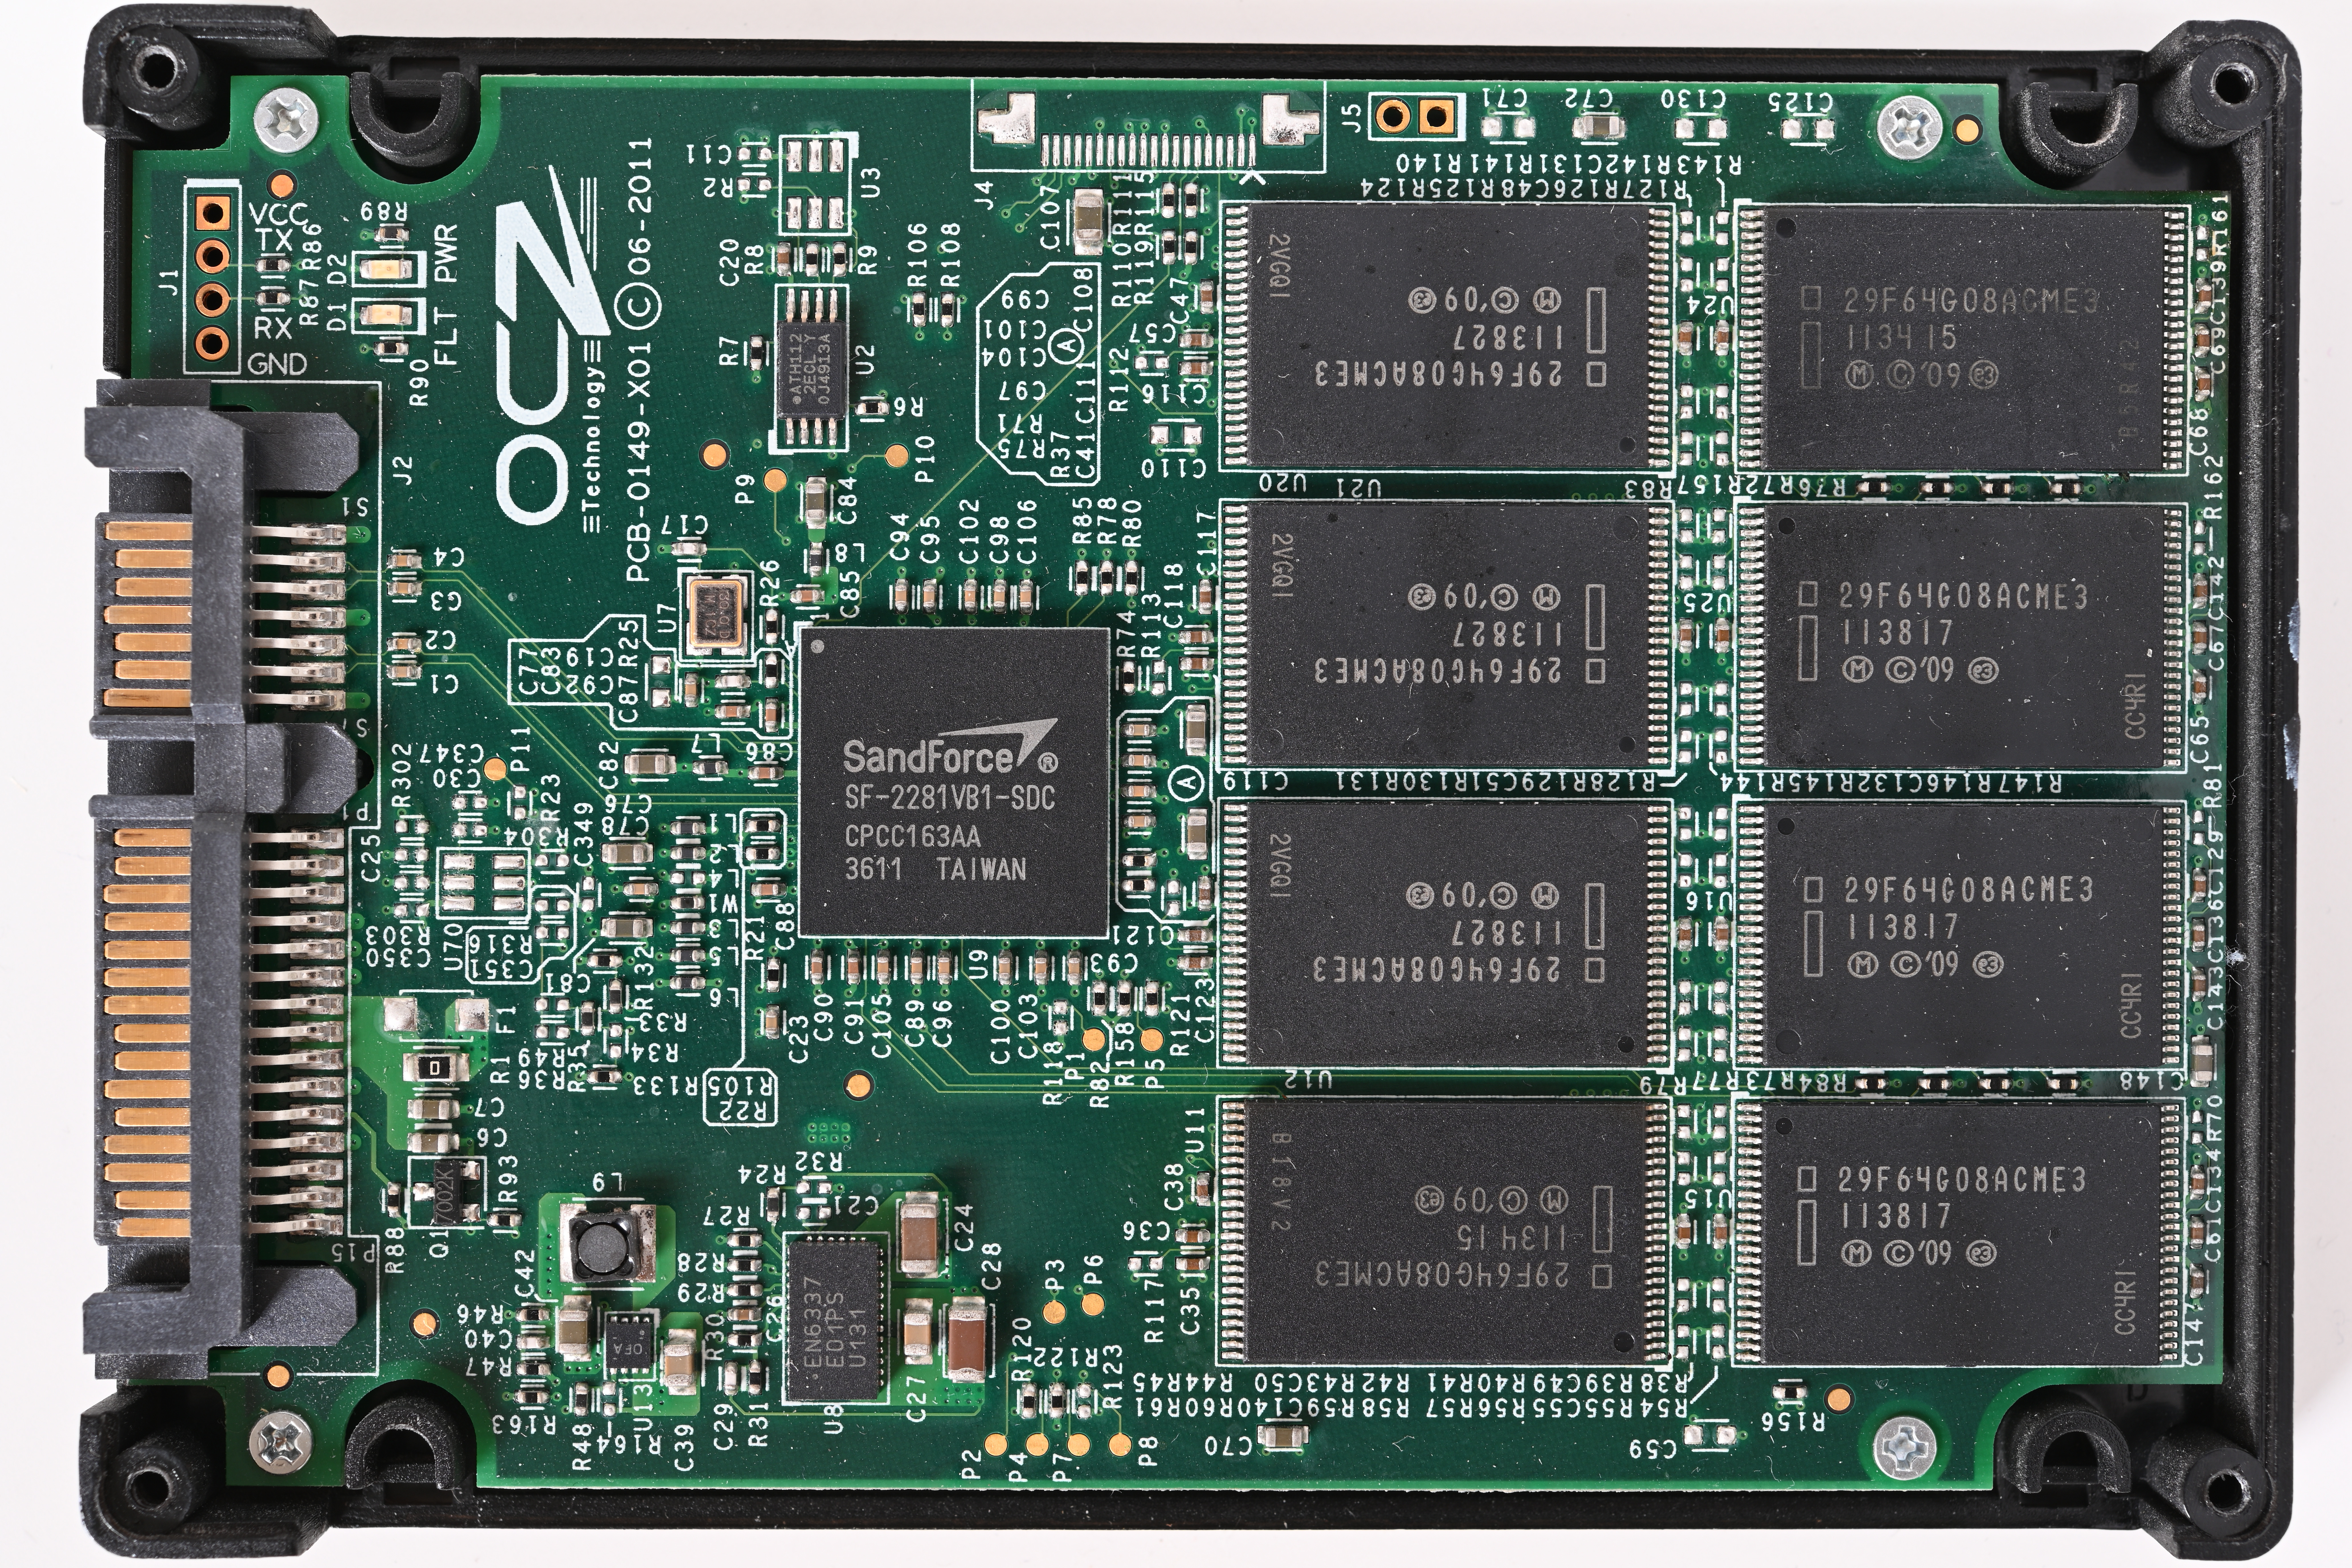
\includegraphics[width=0.88\linewidth,height=3.8cm,keepaspectratio]{Grundlagen_Info/16_ComputerUndKodierungen/Figures/ssd_inside.jpg}
        \caption{Geöffnete \gls{SSD}: Platine mit Speichercontroller und Flash-Chips (keine Mechanik). \href{https://commons.wikimedia.org/wiki/File:OCZ_Agility_3_PCB.jpg}{\color{RoyalBlue}\scriptsize[Quelle: Phiarc, CC BY-SA 4.0]}}
        \label{fig:foto_ssd_inside}
    \end{subfigure}
    \caption{Vergleich des internen Aufbaus von Festplatte (\gls{HDD}) und Solid State Drive (\gls{SSD}).}
    \label{fig:hdd_ssd_aufbau}
\end{figure}

\subsection{Vergleich von Geschwindigkeit und Latenz}

Der fundamentale Unterschied im Aufbau führt zu drastischen Leistungsunterschieden bei zwei zentralen Messgrössen:
\begin{enumerate}
    \item \textbf{Zugriffszeit (Latenz):} Die Zeitverzögerung, bis der Speicher den ersten angeforderten Datenblock liefert. Bei einer \gls{HDD} muss der Arm physisch zur passenden Spur fahren (\emph{Seek-Time}) und warten, bis die rotierende Scheibe den richtigen Sektor unter den Kopf dreht ($5\text{--}15\,\mathrm{ms}$). Eine \gls{SSD} adressiert Flash-Zellen rein elektronisch ($0.02\text{--}0.1\,\mathrm{ms}$), was Zugriffe um den Faktor \textbf{ca.\ 200 beschleunigt}.
    \item \textbf{Datendurchsatz (Übertragungsrate):} Die kontinuierliche Datenmenge pro Sekunde beim Lesen oder Schreiben grösserer zusammenhängender Dateien.
\end{enumerate}

\begin{figure}[H]
    \centering
    \resizebox{\textwidth}{!}{%
        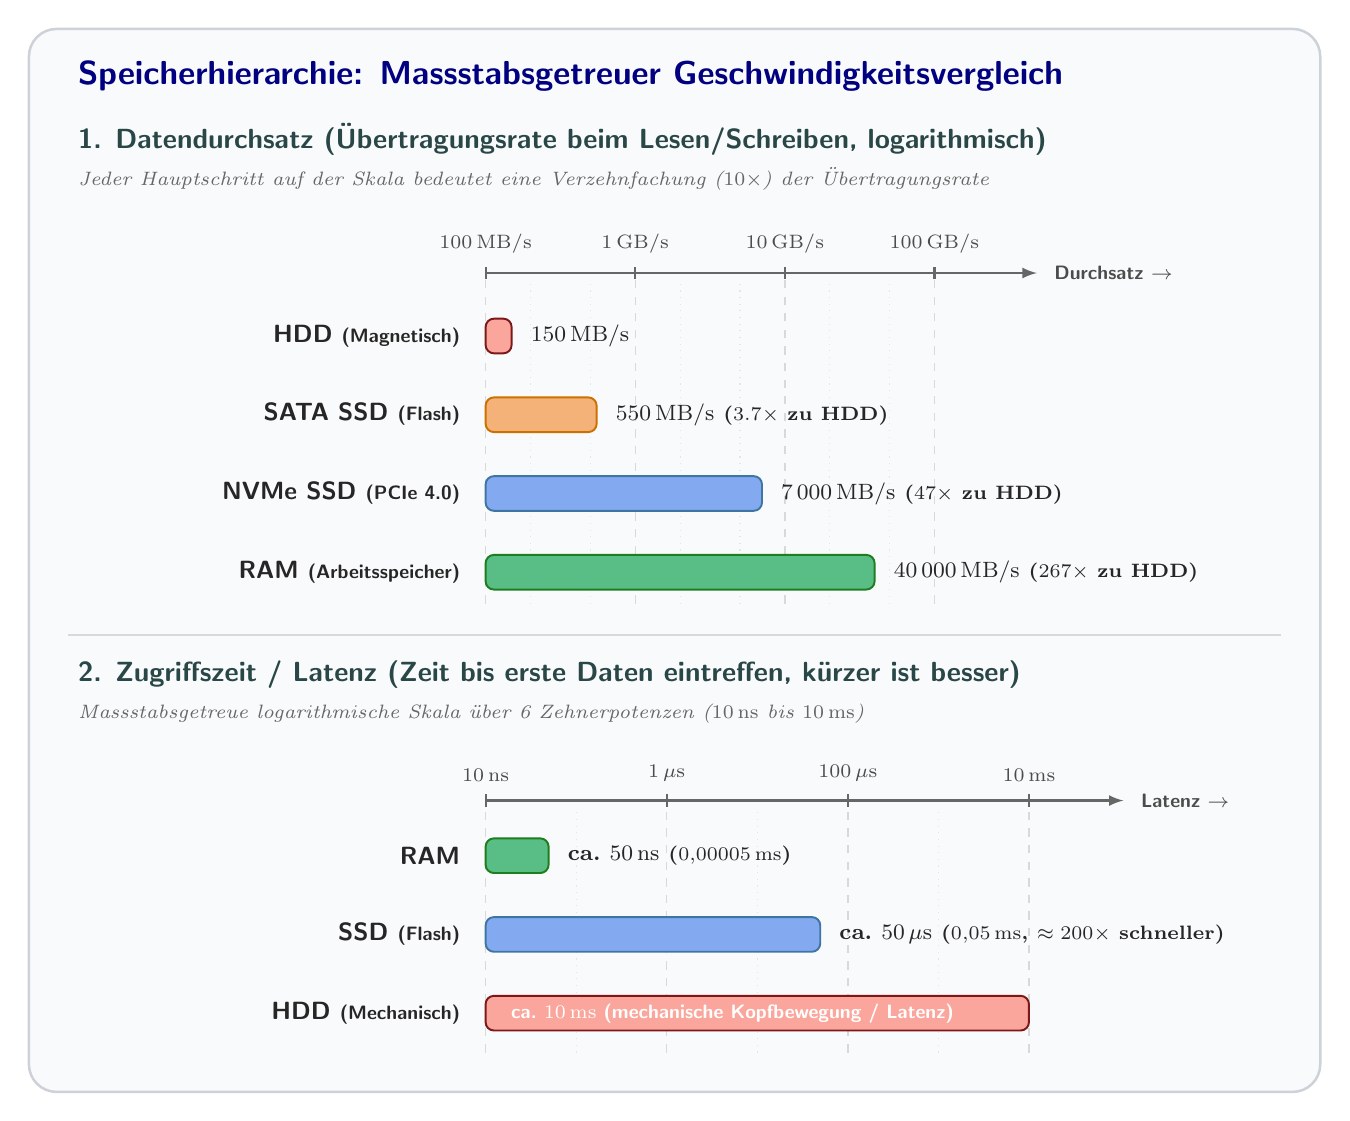
\begin{tikzpicture}[
    font=\small,
    >=latex,
    x=1cm, y=1cm,
    bar/.style={rounded corners=3pt, line width=0.7pt},
    gridline/.style={draw=black!15, dashed, line width=0.5pt},
    labelnode/.style={font=\bfseries\small\sffamily, text=black!85},
    valnode/.style={font=\bfseries\footnotesize, text=black!85}
]

    % Background container (ample padding on left and right)
    \fill[rounded corners=10pt, fill=SlateGray!4, draw=SlateGray!35, line width=0.9pt] (-2.2, -6.6) rectangle (14.2, 6.9);

    % Title
    \node[anchor=west, font=\large\bfseries\sffamily, text=Navy] at (-1.7, 6.3) {Speicherhierarchie: Massstabsgetreuer Geschwindigkeitsvergleich};

    % =========================================================================
    % SECTION 1: DATENDURCHSATZ (Logarithmic Scale)
    % =========================================================================
    \node[anchor=west, font=\bfseries\normalsize\sffamily, text=DarkSlateGray!90!black] at (-1.7, 5.5) {1. Datendurchsatz (Übertragungsrate beim Lesen/Schreiben, logarithmisch)};
    \node[anchor=west, font=\itshape\scriptsize, text=black!60] at (-1.7, 5.0) {Jeder Hauptschritt auf der Skala bedeutet eine Verzehnfachung ($10\times$) der Übertragungsrate};

    % Log Scale: x(v) = 3.60 + 1.90 * log10(v / 100)
    % 100 MB/s    -> 3.60
    % 1 GB/s      -> 5.50
    % 10 GB/s     -> 7.40
    % 100 GB/s    -> 9.30

    % Gridlines & Major Ticks
    \draw[gridline] (3.60, -0.4) -- (3.60, 3.8);
    \draw[gridline] (5.50, -0.4) -- (5.50, 3.8);
    \draw[gridline] (7.40, -0.4) -- (7.40, 3.8);
    \draw[gridline] (9.30, -0.4) -- (9.30, 3.8);

    % Minor gridlines (dotted)
    \foreach \x in {4.17, 4.93, 6.07, 6.83, 7.97, 8.73} {
        \draw[draw=black!10, dotted, line width=0.4pt] (\x, -0.4) -- (\x, 3.7);
    }

    % Axis Line with ticks
    \draw[->, thick, color=black!60] (3.6, 3.8) -- (10.6, 3.8);
    \node[anchor=west, font=\scriptsize\bfseries\sffamily, text=black!70] at (10.7, 3.8) {Durchsatz $\rightarrow$};

    \foreach \x/\lbl in {3.60/{100\,\mathrm{MB/s}}, 5.50/{1\,\mathrm{GB/s}}, 7.40/{10\,\mathrm{GB/s}}, 9.30/{100\,\mathrm{GB/s}}} {
        \draw[black!60, line width=0.8pt] (\x, 3.72) -- (\x, 3.88);
        \node[anchor=south, font=\scriptsize\bfseries, text=black!70] at (\x, 3.92) {$\lbl$};
    }

    % HDD Bar: 150 MB/s -> 3.60 + 1.90*log10(1.5) = 3.93
    \node[anchor=east, labelnode] at (3.4, 3.0) {HDD \scriptsize(Magnetisch)};
    \fill[bar, fill=Salmon!70, draw=FireBrick!70!black] (3.60, 2.78) rectangle (3.93, 3.22);
    \node[anchor=west, valnode] at (4.05, 3.0) {$150\,\mathrm{MB/s}$};

    % SATA SSD Bar: 550 MB/s -> 3.60 + 1.90*log10(5.5) = 5.01
    \node[anchor=east, labelnode] at (3.4, 2.0) {SATA SSD \scriptsize(Flash)};
    \fill[bar, fill=SandyBrown!85, draw=DarkOrange!80!black] (3.60, 1.78) rectangle (5.01, 2.22);
    \node[anchor=west, valnode] at (5.13, 2.0) {$550\,\mathrm{MB/s}$ \scriptsize(\textbf{$3.7\times$} zu HDD)};

    % NVMe SSD Bar: 7000 MB/s -> 3.60 + 1.90*log10(70) = 7.11
    \node[anchor=east, labelnode] at (3.4, 1.0) {NVMe SSD \scriptsize(PCIe 4.0)};
    \fill[bar, fill=CornflowerBlue!80, draw=SteelBlue!90!black] (3.60, 0.78) rectangle (7.11, 1.22);
    \node[anchor=west, valnode] at (7.23, 1.0) {$7\,000\,\mathrm{MB/s}$ \scriptsize(\textbf{$47\times$} zu HDD)};

    % RAM Bar: 40000 MB/s -> 3.60 + 1.90*log10(400) = 8.54
    \node[anchor=east, labelnode] at (3.4, 0.0) {RAM \scriptsize(Arbeitsspeicher)};
    \fill[bar, fill=MediumSeaGreen!85, draw=ForestGreen!90!black] (3.60, -0.22) rectangle (8.54, 0.22);
    \node[anchor=west, valnode] at (8.66, 0.0) {$40\,000\,\mathrm{MB/s}$ \scriptsize(\textbf{$267\times$} zu HDD)};


    % =========================================================================
    % SECTION 2: ZUGRIFFSZEIT / LATENZ (Logarithmic Scale)
    % =========================================================================
    \draw[thick, color=black!15] (-1.7, -0.8) -- (13.7, -0.8);
    \node[anchor=west, font=\bfseries\normalsize\sffamily, text=DarkSlateGray!90!black] at (-1.7, -1.3) {2. Zugriffszeit / Latenz (Zeit bis erste Daten eintreffen, kürzer ist besser)};
    \node[anchor=west, font=\itshape\scriptsize, text=black!60] at (-1.7, -1.8) {Massstabsgetreue logarithmische Skala über 6 Zehnerpotenzen ($10\,\mathrm{ns}$ bis $10\,\mathrm{ms}$)};

    % Latency Scale: 6 decades from 10ns to 10ms -> 1.15 cm per decade
    % x(t) = 3.60 + 1.15 * log10(t / 10ns)
    % 10 ns   -> 3.60
    % 100 ns  -> 4.75
    % 1 us    -> 5.90
    % 10 us   -> 7.05
    % 100 us  -> 8.20
    % 1 ms    -> 9.35
    % 10 ms   -> 10.50

    % Gridlines for latency
    \draw[gridline] (3.60, -6.1) -- (3.60, -2.9);
    \draw[gridline] (5.90, -6.1) -- (5.90, -2.9);
    \draw[gridline] (8.20, -6.1) -- (8.20, -2.9);
    \draw[gridline] (10.50, -6.1) -- (10.50, -2.9);

    % Minor gridlines for latency
    \foreach \x in {4.75, 7.05, 9.35} {
        \draw[draw=black!10, dotted, line width=0.4pt] (\x, -6.1) -- (\x, -3.0);
    }

    % Axis line with ticks
    \draw[->, thick, color=black!60] (3.6, -2.9) -- (11.7, -2.9);
    \node[anchor=west, font=\scriptsize\bfseries\sffamily, text=black!70] at (11.8, -2.9) {Latenz $\rightarrow$};

    \foreach \x/\lbl in {3.60/{10\,\mathrm{ns}}, 5.90/{1\,\mu\mathrm{s}}, 8.20/{100\,\mu\mathrm{s}}, 10.50/{10\,\mathrm{ms}}} {
        \draw[black!60, line width=0.8pt] (\x, -2.98) -- (\x, -2.82);
        \node[anchor=south, font=\scriptsize\bfseries, text=black!70] at (\x, -2.78) {$\lbl$};
    }

    % RAM Latency: 50 ns -> 3.60 + 1.15*log10(5) = 4.40
    \node[anchor=east, labelnode] at (3.4, -3.6) {RAM};
    \fill[bar, fill=MediumSeaGreen!85, draw=ForestGreen!90!black] (3.60, -3.82) rectangle (4.40, -3.38);
    \node[anchor=west, valnode] at (4.52, -3.6) {ca.\ $50\,\mathrm{ns}$ \scriptsize($0{,}00005\,\mathrm{ms}$)};

    % SSD Latency: 50 us -> 3.60 + 1.15*log10(5000) = 7.85
    \node[anchor=east, labelnode] at (3.4, -4.6) {SSD \scriptsize(Flash)};
    \fill[bar, fill=CornflowerBlue!80, draw=SteelBlue!90!black] (3.60, -4.82) rectangle (7.85, -4.38);
    \node[anchor=west, valnode] at (7.97, -4.6) {ca.\ $50\,\mu\mathrm{s}$ \scriptsize($0{,}05\,\mathrm{ms}$, \textbf{$\approx 200\times$} schneller)};

    % HDD Latency: 10 ms (10^7 ns) -> 3.60 + 1.15*6 = 10.50
    \node[anchor=east, labelnode] at (3.4, -5.6) {HDD \scriptsize(Mechanisch)};
    \fill[bar, fill=Salmon!70, draw=FireBrick!70!black] (3.60, -5.82) rectangle (10.50, -5.38);
    % Inset label inside bar
    \node[anchor=west, font=\bfseries\scriptsize\sffamily, text=white] at (3.80, -5.6) {ca.\ $10\,\mathrm{ms}$ (mechanische Kopfbewegung / Latenz)};

\end{tikzpicture}

    }
    \caption{Übertragungsraten und Zugriffszeiten im direkten Vergleich zwischen \gls{HDD}, \gls{SSD} und \gls{RAM}.}
    \label{fig:speed_vergleich}
\end{figure}

\begin{myexample}[Speicherhierarchie und Kosten]
    Der \gls{RAM} eines modernen Computers kann Daten mit Übertragungsraten von 30--50~GB/s lesen. Eine \gls{NVMe}-\gls{SSD} schafft bis zu 7~GB/s, eine ältere \gls{SATA}-\gls{SSD} ca.\ 550~MB/s und eine herkömmliche mechanische \gls{HDD} nur ca.\ 100--200~MB/s.

    \textbf{Faustregel: Je schneller der Speicher, desto teurer ist er in der Regel pro Gigabyte.} Deshalb kombiniert ein Computer verschiedene Speicherarten hierarchisch: extrem schnellen, aber teuren und flüchtigen \gls{RAM} für aktuell laufende Prozesse und günstigeren Massenspeicher für die dauerhafte Ablage grosser Datenmengen.
\end{myexample}

\begin{myexercise}\label{myexercise:foto-laden-ssd-hdd}
    \textbf{Foto laden: \gls{SSD} vs.\ \gls{HDD} und die Rolle des Arbeitsspeichers.}
    Ein hochauflösendes Foto mit einer Grösse von $24\,\mathrm{MB}$ soll in ein Bildbearbeitungsprogramm geladen werden. Für die Speicherarten gelten folgende Kennwerte:
    \begin{itemize}
        \item \textbf{\gls{SSD}:} Lesegeschwindigkeit $2\,\mathrm{GB/s} = 2000\,\mathrm{MB/s}$, Zugriffszeit (Latenz) $0{,}05\,\mathrm{ms}$.
        \item \textbf{\gls{HDD}:} Lesegeschwindigkeit $150\,\mathrm{MB/s}$, Zugriffszeit (Latenz) $10\,\mathrm{ms}$.
        \item \textbf{\gls{RAM}:} Übertragungsrate $40\,\mathrm{GB/s}$, Latenz $0{,}00005\,\mathrm{ms}$.
    \end{itemize}

    \begin{enumerate}[(a)]
        \item \textbf{Reine Übertragungsdauer:} Wie lange dauert das reine serielle Einlesen des 24-MB-Fotos auf der \gls{SSD} im Vergleich zur herkömmlichen \gls{HDD}? ($t=\frac{\text{Datenmenge}}{\text{Lesegeschwindigkeit}}$).
        \item \textbf{Einfluss der Latenz:} Vor der Datenübertragung muss der Speicher den ersten Block adressieren (Zugriffszeit). Berechnen Sie die Gesamtdauer ($t_\text{gesamt} = t_\text{Latenz} + t_\text{Übertragung}$) für \gls{SSD} und \gls{HDD}.
        \item \textbf{Viele kleine Dateien:} Nun soll kein einzelnes Foto geladen werden, sondern eine Thumbnail-Vorschau aus \textbf{1'000 kleinen Mini-Bildern} zu je $24\,\mathrm{kB}$ (Gesamtmenge ebenfalls $24\,\mathrm{MB}$). Für jedes Bild fällt erneut die volle Zugriffszeit an ($t_\text{gesamt} = 1000 \times t_\text{Latenz} + t_\text{Übertragung}$). Wie lange dauert das Laden auf \gls{SSD} und auf \gls{HDD}? Warum bricht die \gls{HDD} hier so massiv ein?
        \item \textbf{Zielort der Daten:} Wohin genau fliessen die Daten beim \enquote{Öffnen} des Fotos, und warum kann die \gls{CPU} das Bild nicht einfach direkt auf der \gls{SSD} bearbeiten?
        \item \textbf{Speichern und Flüchtigkeit:} Sie bearbeiten das geöffnete Bild über längere Zeit. Was passiert bei einem plötzlichen Stromausfall, wenn Sie noch nicht auf \enquote{Speichern} gedrückt haben? Begründen Sie mit den physikalischen Eigenschaften von \gls{RAM} und Massenspeicher.
    \end{enumerate}

    \begin{myanswer}
        \begin{enumerate}[(a)]
            \item \textbf{Reine Übertragungsdauer:}
            \begin{itemize}
                \item \textbf{\gls{SSD}:} $\dfrac{24\,\mathrm{MB}}{2000\,\mathrm{MB/s}} = 0{,}012\,\mathrm{s} = 12\,\mathrm{ms}$.
                \item \textbf{\gls{HDD}:} $\dfrac{24\,\mathrm{MB}}{150\,\mathrm{MB/s}} = 0{,}160\,\mathrm{s} = 160\,\mathrm{ms}$ (über $13\times$ langsamer).
            \end{itemize}
            \item \textbf{Gesamtdauer bei einer einzelnen Datei:}
            \begin{itemize}
                \item \textbf{\gls{SSD}:} $0{,}05\,\mathrm{ms} + 12\,\mathrm{ms} = 12{,}05\,\mathrm{ms} \approx 0{,}012\,\mathrm{s}$.
                \item \textbf{\gls{HDD}:} $10\,\mathrm{ms} + 160\,\mathrm{ms} = 170\,\mathrm{ms} = 0{,}17\,\mathrm{s}$.
            \end{itemize}
            \item \textbf{1'000 kleine Dateien (Thumbnail-Galerie):}
            \begin{itemize}
                \item \textbf{\gls{SSD}:} $1000 \times 0{,}05\,\mathrm{ms} + 12\,\mathrm{ms} = 50\,\mathrm{ms} + 12\,\mathrm{ms} = 62\,\mathrm{ms} \approx 0{,}06\,\mathrm{s}$ (praktisch verzögerungsfrei).
                \item \textbf{\gls{HDD}:} $1000 \times 10\,\mathrm{ms} + 160\,\mathrm{ms} = 10\,000\,\mathrm{ms} + 160\,\mathrm{ms} = 10{,}16\,\mathrm{s}$ (über 10 Sekunden Wartezeit!).
                \item \textbf{Begründung:} Bei der \gls{HDD} muss der mechanische Lese-/Schreibarm für jedes einzelne Bild neu positioniert werden und auf die rotierende Scheibe warten (\emph{Seek-Time}). Bei der \gls{SSD} erfolgt der Zugriff rein elektronisch in Mikrosekunden.
            \end{itemize}
            \item \textbf{Zielort:} Die Daten werden vom Massenspeicher (\gls{SSD}/\gls{HDD}) in den \textbf{Arbeitsspeicher (\gls{RAM})} kopiert. Die \gls{CPU} kann Befehle nur im \gls{RAM} und in ihren eigenen Registern mit voller Busgeschwindigkeit ($40\,\mathrm{GB/s}$) und Nanosekunden-Latenz abarbeiten; Massenspeicher wäre für die laufende Bildberechnung viel zu langsam.
            \item \textbf{Stromausfall:} Alle noch nicht gespeicherten Bearbeitungsschritte gehen verloren. Der \gls{RAM} ist ein \emph{flüchtiger} Speicher, dessen Inhalt ohne Versorgungsspannung sofort gelöscht wird. Erst beim Speichern werden die Bilddaten über das Dateisystem dauerhaft auf den \emph{nicht-flüchtigen} Massenspeicher (\gls{SSD}/\gls{HDD}) geschrieben.
        \end{enumerate}
    \end{myanswer}
\end{myexercise}

\begin{myexercise}\label{myexercise:steam-speicherzeit}
    \textbf{Ein neues Game von Steam herunterladen.}
    Sie möchten ein Game mit einer Downloadgrösse von 120~GB herunterladen. Stellen Sie sich vor, die Download-Geschwindigkeit sei unbegrenzt: Nur die Schreibgeschwindigkeit des Zielspeichers begrenzt, wie schnell die Daten gespeichert werden können.

    Verwenden Sie für dieses vereinfachte Rechenmodell die folgenden konstanten \emph{Schreibgeschwindigkeiten}. Auf jedem Speicher stehen mindestens 120~GB frei, auch beim hier angenommenen \gls{RAM}. Entpacken und Installation werden nicht berücksichtigt. Rechnen Sie mit $1\,\mathrm{GB}=1000\,\mathrm{MB}$.
    \begin{center}
        \begin{tabular}{lc}
            Speicher & Angenommene Schreibgeschwindigkeit \\ \midrule
            \gls{RAM} & $40\,\mathrm{GB/s}$ \\
            \gls{SSD} & $2\,\mathrm{GB/s}$ \\
            \gls{HDD} & $150\,\mathrm{MB/s}$ \\
        \end{tabular}
    \end{center}
    \begin{enumerate}[(a)]
        \item Wie lange dauert das reine Speichern der 120~GB jeweils in \gls{RAM}, auf \gls{SSD} und auf \gls{HDD}? Geben Sie die Zeiten in Sekunden und, wo sinnvoll, in Minuten an. Nutzen Sie $t=\frac{\text{Datenmenge}}{\text{Schreibgeschwindigkeit}}$.
        \item Der \gls{RAM} ist am schnellsten. Warum ist er trotzdem keine geeignete dauerhafte Ablage für das heruntergeladene Game?
    \end{enumerate}
    \begin{myanswer}
        \begin{enumerate}[(a)]
            \item Die Datenmenge beträgt $120\,\mathrm{GB}=120\,000\,\mathrm{MB}$.
            \begin{itemize}
                \item \textbf{\gls{RAM}:} $\frac{120\,\mathrm{GB}}{40\,\mathrm{GB/s}}=3\,\mathrm{s}$.
                \item \textbf{\gls{SSD}:} $\frac{120\,\mathrm{GB}}{2\,\mathrm{GB/s}}=60\,\mathrm{s}=1\,\mathrm{min}$.
                \item \textbf{\gls{HDD}:} $\frac{120\,000\,\mathrm{MB}}{150\,\mathrm{MB/s}}=800\,\mathrm{s}=13\,\mathrm{min}\,20\,\mathrm{s}$.
            \end{itemize}
            \item \gls{RAM} ist flüchtig: Beim Ausschalten gehen die Daten verloren. \gls{SSD} und \gls{HDD} behalten sie auch ohne Strom. Die berechneten Zeiten betreffen nur das Schreiben der Daten im vereinfachten Modell; sie sind keine Vorhersage der gesamten Download- und Installationsdauer. Nicht zuletzt verfügen die meisten Computer über deutlich weniger \gls{RAM} als 120~GB, sodass das Game gar nicht in den \gls{RAM} passen würde.
        \end{enumerate}
    \end{myanswer}
\end{myexercise}

\section{Der Fetch-Decode-Execute-Zyklus}\label{sec:fde}

Die \gls{CPU} führt Anweisungen in einem einfachen, immer wiederholten Schema aus, dem \tib{Fetch-Decode-Execute-Zyklus}\index{Fetch-Decode-Execute-Zyklus}:

\begin{figure}[H]
    \centering
    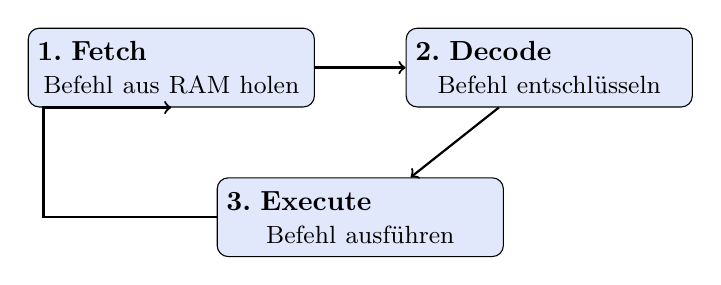
\begin{tikzpicture}[
    block/.style={draw, rounded corners, minimum width=3.4cm, minimum height=1.0cm, text centered, text width=3.4cm, fill=RoyalBlue!15},
    arrow/.style={->, thick}
]
    \node[block] (fetch)   at (0, 0)    {\textbf{1.\ Fetch} \newline \small Befehl aus RAM holen};
    \node[block] (decode)  at (4.8, 0)  {\textbf{2.\ Decode} \newline \small Befehl entschlüsseln};
    \node[block] (execute) at (2.4,-1.9) {\textbf{3.\ Execute} \newline \small Befehl ausführen};

    \draw[arrow] (fetch)   -- (decode);
    \draw[arrow] (decode)  -- (execute);
    \draw[arrow] (execute.west) -- ++(-2.2,0) |- (fetch.south);
\end{tikzpicture}

    \caption{Der Fetch-Decode-Execute-Zyklus: die \gls{CPU} wiederholt diesen Ablauf Milliarden Mal pro Sekunde.}
    \label{fig:fde}
\end{figure}

\begin{enumerate}
    \item \tib{Fetch}\index{Fetch-Decode-Execute-Zyklus!Fetch} (Holen): Das Steuerwerk liest den nächsten Befehl aus dem \gls{RAM} an der Adresse, auf die der \emph{Programmzähler} (engl.\ \emph{program counter}) zeigt.
    \item \tib{Decode}\index{Fetch-Decode-Execute-Zyklus!Decode} (Dekodieren): Der Befehl wird in seine Bestandteile zerlegt: \emph{Was ist zu tun?} (Operationscode, z.\,B. Addieren) und \emph{Mit welchen Daten?} (Operanden, z.\,B. Register R1 und R2).
    \item \tib{Execute}\index{Fetch-Decode-Execute-Zyklus!Execute} (Ausführen): Die \gls{ALU} oder eine andere Komponente führt die Anweisung aus (z.\,B. Addition), das Ergebnis wird in ein Register oder in den \gls{RAM} geschrieben, und der Programmzähler rückt weiter.
\end{enumerate}

\begin{myexample}[Konkreter Ablauf eines \gls{FDE}-Zyklus]
    Angenommen, im Register \texttt{R1} steht der Wert $3$, im Register \texttt{R2} der Wert $5$, und an Speicheradresse \texttt{100} liegt der Maschinenbefehl \texttt{ADD R1, R2}:
    \begin{itemize}
        \item \textbf{Fetch:} Der Programmzähler steht auf Adresse \texttt{100}. Das Steuerwerk liest das Binärmuster dieses Befehls aus dem \gls{RAM} in das Befehlsregister der \gls{CPU}. Gleichzeitig wird der Programmzähler auf die nächste Adresse (\texttt{101}) vorbereitet.
        \item \textbf{Decode:} Das Steuerwerk entschlüsselt das Bitmuster. Es erkennt: \enquote{Operation: Addition; Operand 1: Register \texttt{R1}; Operand 2: Register \texttt{R2}; Ziel: Register \texttt{R1}}.
        \item \textbf{Execute:} Die \gls{ALU} schaltet die Werte der beiden Register an ihre Eingänge, berechnet $3 + 5 = 8$ und speichert das Ergebnis $8$ zurück in das Register \texttt{R1}. Der Zyklus ist abgeschlossen.
    \end{itemize}
\end{myexample}

\subsection{Taktfrequenz und die Einheit Hertz (Hz)}

Damit alle Komponenten einer \gls{CPU} synchron zusammenarbeiten, gibt ein elektronischer Taktgeber einen gleichmässigen Rhythmus vor -- wie der Schrittmacher eines Orchesters.

Die Geschwindigkeit dieses Takts heisst \tib{Taktfrequenz}\index{Taktfrequenz} und wird in der physikalischen Einheit \tib{Hertz (Hz)}\index{Hertz (Hz)} gemessen:
\[
    1\,\mathrm{Hz} = 1\text{ Takt bzw. Schwingung pro Sekunde}\quad (1\,\mathrm{s}^{-1}).
\]
Heutige Prozessoren arbeiten im Gigahertz-Bereich:
\begin{center}
    \begin{tabular}{lll}
        Einheit & Bedeutung & Takte pro Sekunde \\\midrule\midrule
        $1\,\mathrm{kHz}$ (Kilohertz) & Tausend Takte & $10^3 = 1\,000\,\mathrm{Hz}$ \\\midrule
        $1\,\mathrm{MHz}$ (Megahertz) & Million Takte & $10^6 = 1\,000\,000\,\mathrm{Hz}$ \\\midrule
        $1\,\mathrm{GHz}$ (Gigahertz) & Milliarde Takte & $10^9 = 1\,000\,000\,000\,\mathrm{Hz}$ \\
    \end{tabular}
\end{center}
Ein Prozessor mit einer Taktfrequenz von $3{,}6\,\mathrm{GHz}$ durchläuft $3{,}6$ Milliarden Taktzyklen pro Sekunde. Je nach Prozessorarchitektur benötigt ein Befehl einen oder mehrere Taktzyklen, oder moderne \glspl{CPU} führen durch parallele Einheiten (Pipelining, Mehrkernprozessoren) sogar mehrere Befehle pro Taktzyklus aus.


\begin{myexercise}
    Ein Prozessor hat eine Taktfrequenz von $3{,}6\,\mathrm{GHz}$ und führt im Durchschnitt 2 Befehle pro Taktzyklus aus.
    \begin{enumerate}
        \item Wie viele Befehle führt der Prozessor pro Sekunde aus?
        \item Ein Programm besteht aus $7{,}2 \times 10^9$ Befehlen. Wie lange dauert die Ausführung?
    \end{enumerate}
    \begin{myanswer}
        \begin{enumerate}
            \item $3{,}6 \times 10^9 \,\mathrm{Hz} \times 2 = 7{,}2 \times 10^9$ Befehle pro Sekunde.
            \item $\dfrac{7{,}2 \times 10^9}{7{,}2 \times 10^9\,\mathrm{s}^{-1}} = 1\,\mathrm{s}$.
        \end{enumerate}
    \end{myanswer}
\end{myexercise}

\begin{mychallenge}
    Der Addierbefehl \texttt{ADD R1, R2} weist die \gls{CPU} an, den Inhalt der Register \texttt{R1} und \texttt{R2} zu addieren. Ordnen Sie die folgenden Teilschritte den drei Phasen Fetch, Decode und Execute zu:
    \begin{itemize}
        \item Der Programmzähler wird um eine Stelle weitergeschaltet.
        \item Die \gls{ALU} berechnet die Summe der beiden Register.
        \item Das Steuerwerk erkennt, dass es sich um einen Additionsbefehl mit zwei Registeroperanden handelt.
        \item Der Befehl \texttt{ADD R1, R2} wird als Bitfolge aus dem \gls{RAM} gelesen.
    \end{itemize}
    \begin{myanswer}
        \begin{itemize}
            \item Befehl aus \gls{RAM} lesen $\to$ Fetch
            \item Programmzähler weiterschalten $\to$ Fetch
            \item Befehl als Additionsbefehl mit zwei Registeroperanden erkennen $\to$ Decode
            \item \gls{ALU} berechnet Summe $\to$ Execute
        \end{itemize}
    \end{myanswer}
\end{mychallenge}

Wir haben nun gesehen, wie \gls{CPU}, Arbeitsspeicher, Massenspeicher und Ein-/Ausgabe zusammenspielen, um Programme auszuführen. Im nächsten Kapitel betrachten wir, wie das Betriebssystem diese Hardware-Ressourcen verwaltet und den Anwendungen zugänglich macht.
